\begin{center}
	\begin{circuitfig}[H]
		\centering
		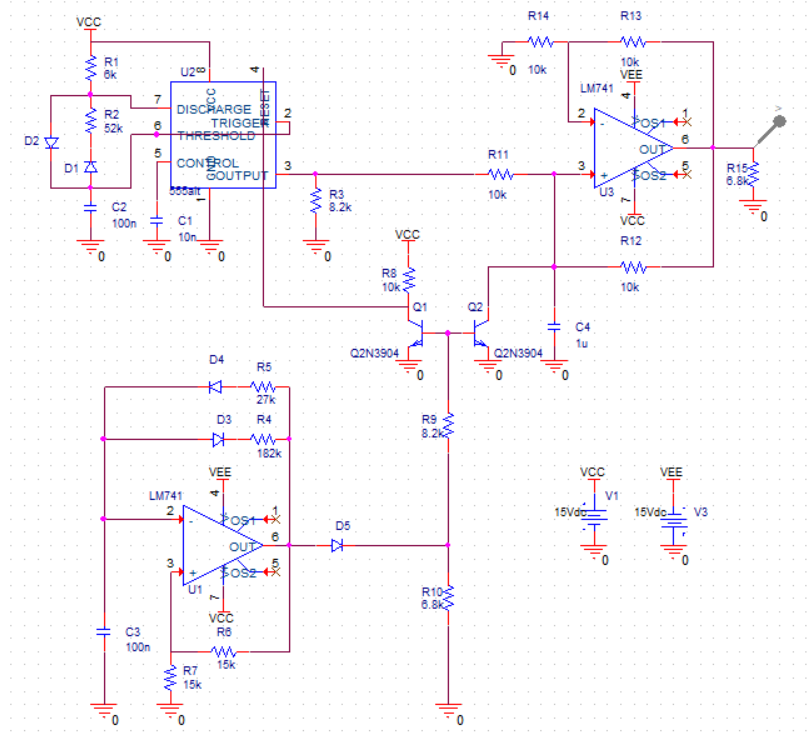
\includegraphics[width=10cm]{spice_02/lab 2 circuit}
		\caption{Κύκλωμα προσομοίωσης για το PSpice.}
		\label{circ:2_schematik}
	\end{circuitfig}
\end{center}

Οι προσομοιώσεις έγιναν με το κύκλωμα 2.2. Οι πρώτες δύο δείχνουν τις εξόδους των ταλαντωτών Α και Β, όταν δεν είναι συνδεδεμένοι στον ολοκληρωτή. Η τρίτη απεικονίζει την έξοδο ολόκληρου του κυκλώματος.

\begin{plot_fig}[H]
	\begin{center}
		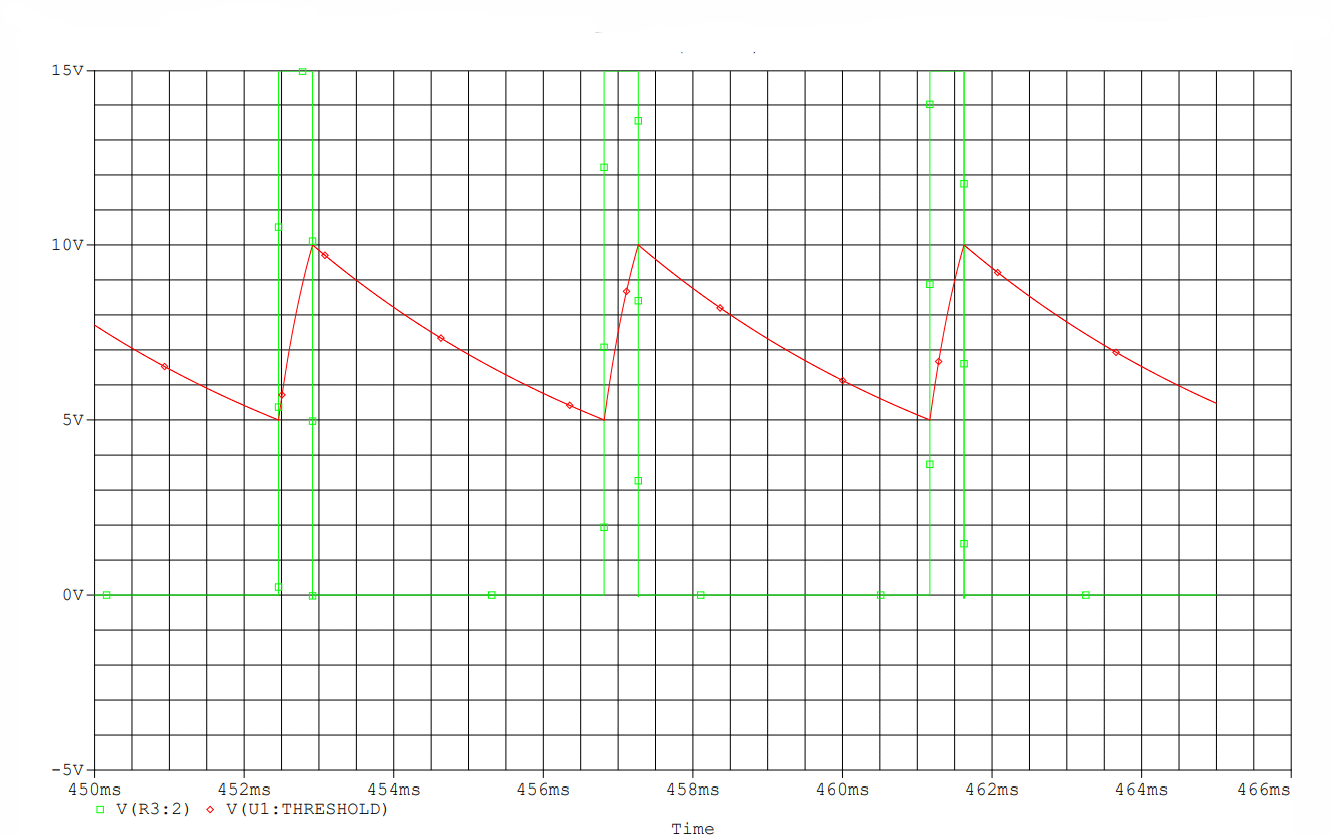
\includegraphics[width=10cm]{spice_02/lab2 q3.1}
		\caption{Οι τάσεις $v_1$ (πράσινη κυματομορφή) στην έξοδο και η τάση του ακροδέκτη 6 (κόκκινη κυματομορφή) του 555.}
		\label{plot:ask2:q3_1}
	\end{center}
\end{plot_fig}

\begin{plot_fig}[H]
	\begin{center}
		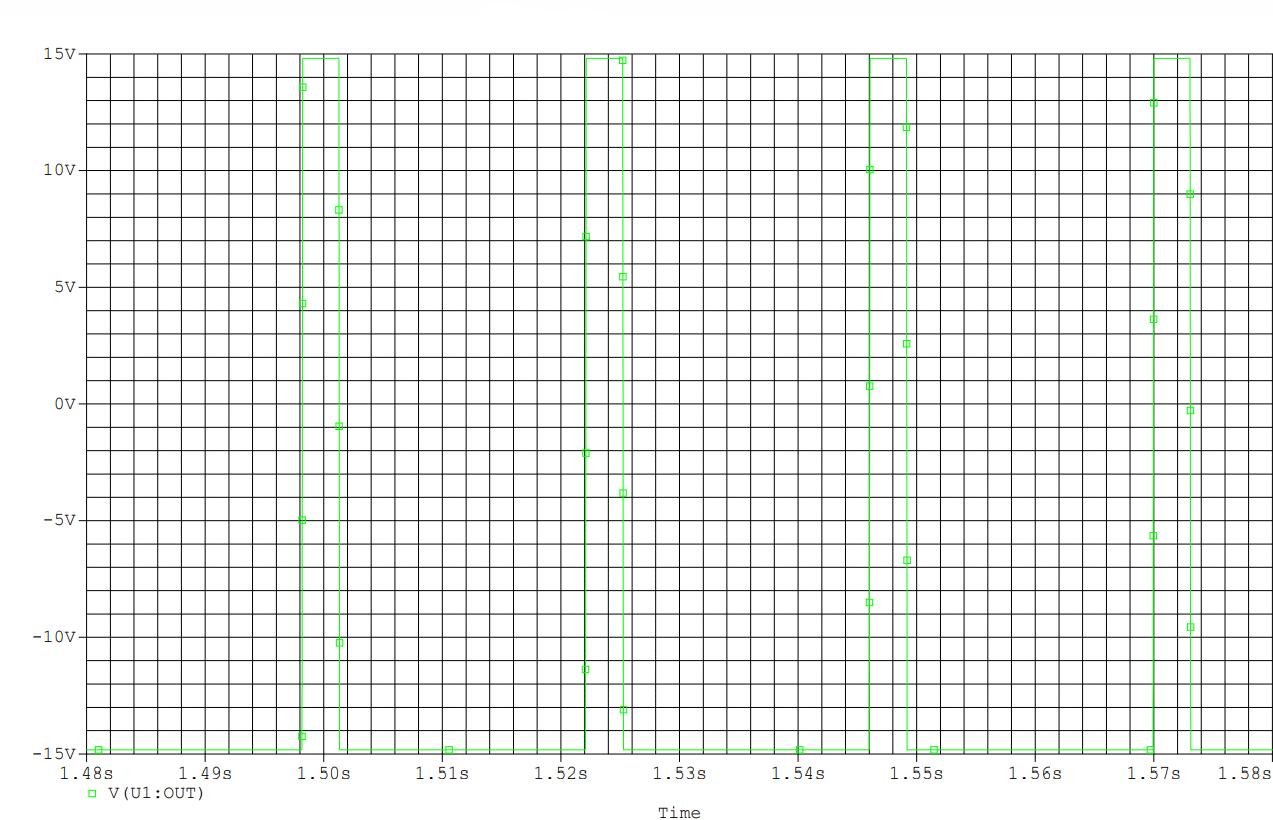
\includegraphics[width=10cm]{spice_02/lab2 q3.2}
		\caption{Η τάση $v_2$ στην έξοδο του ασταθούς ταλαντωτή Β.}
		\label{plot:ask2:q3_2}
	\end{center}
\end{plot_fig}

\begin{plot_fig}[H]
	\begin{center}
		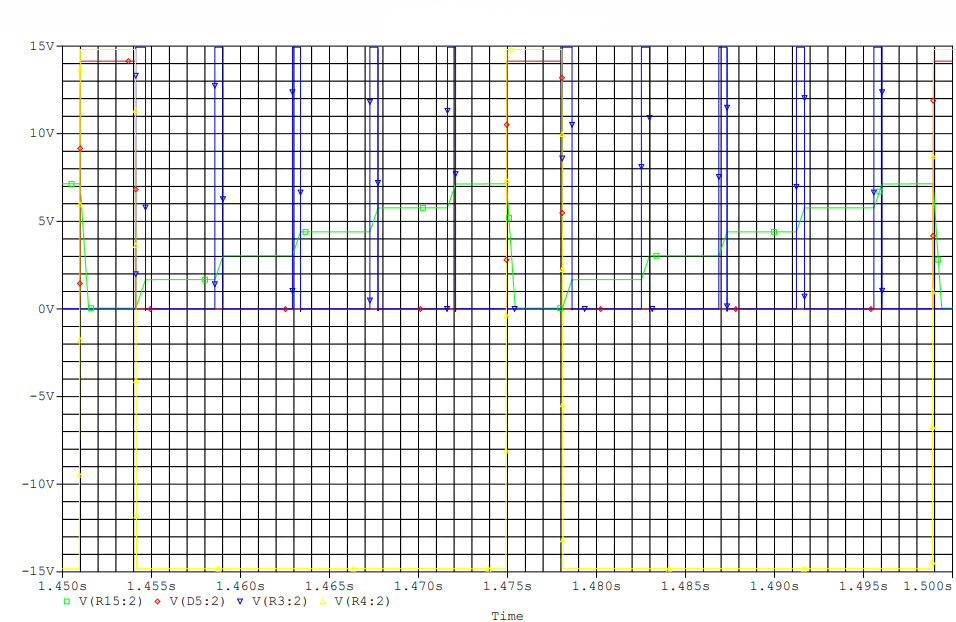
\includegraphics[width=10cm]{spice_02/lab2 q4}
		\caption{Οι τάσεις $v_{\mathrm{out}}$ (πράσινη κυματομορφή) στην έξοδο του ολοκληρωτή, $v_3$ (κόκκινη κυματομορφή) στην κάθοδο της διόδου $D_5$, $v_2$ (κίτρινη κυματομορφή) στην έξοδο του ασταθούς ταλαντωτή Β και $v_1$ (μπλέ κυματομορφή) στην έξοδο του 555.}
		\label{plot:ask2:q4_1}
	\end{center}
\end{plot_fig}